\chapter{Theory and Fundamentals of Passive Cell Balancing}
This chapter explains fundamentals of passive cell balancing and discuss on different types of passive balancing, it's merits, and it's demerits. The chapter also explains the merits of passive balancing technique compared to active balancing technique.


\section{Passive Cell Balancing}
Passive cell balancing is a technique which uses a shunt resistance in order to balance cells in a battery pack. This method is based on dissipating excess energy from higher SOC cell(s) by bypassing the current of the higher SOC cell(s) through a parallel resistance path as shown in the Figure 2.1. Passive balancing is one of the most commonly used balancing methods in EVs due to its simplicity, cost-effectiveness, and small weight and size. Some amount of energy is wasted during balancing process when compared to active cell balancing which is based on sharing charge between the cells but still passive balancing is preferred due its merits. There are two types of passive balancing techniques namely Fixed shunt resistor method and Switching shunt resistor method.

\begin{figure}[h!]
    \centering
    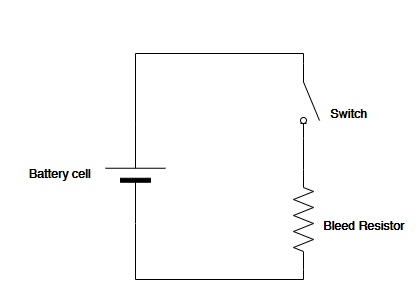
\includegraphics[]{Chapter2/Figures/passivebal.PNG}
    \caption{Passive cell balancing}
\end{figure}

\section{Types of Passive Cell Balancing}
\subsection{Fixed shunt resistor method}
In this technique a fixed  resistance is connected in parallel to every cell in the pack based on required cell balance current. So the excess battery energy is dissipated through the resistor which limits the voltage of each cell in the pack as shown in the Figure 2.2.

This method is suitable for nickel and lead‐acid batteries balancing circuit and not suitable for Li-ion batteries, since these batteries are brought into overcharge conditions without any damage\cite{hemavathi}. This circuit is very simple, hence cost to build one is very less because only resistors are used. But the disadvantage of this technique is constant energy losses and energy is dissipated as heat so brings in need for cooling the system and no control over balancing process.

\begin{figure}[h!]
    \centering
    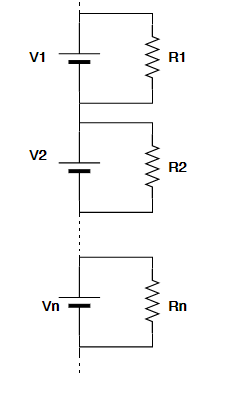
\includegraphics[]{Chapter2/Figures/fixedR.PNG}
    \caption{Fixed shunt resistor method}
\end{figure}

\subsection{Switching shunt resistor method}
Switching shunt resistor method balances each cell voltage using a resistor in parallel with each series connected cell through controlled  semiconductor switches i.e MOSFETs as shown in the Figure 2.3. In this method, the resistor value is properly chooses based on the required balancing current. This method requires a controller for controlling the circuit. At first, voltage of each cell needs to be sensed in and if any cell imbalance is detected suitable decision is to be taken to switch on parallel paths in order to to get the pack balanced.

This method is also called as charge shutting method and is commonly used for Li‐ion batteries balancing circuit. This circuit is more reliable than a fixed shunt resistor balancing circuit. Also, this technique is providing the energy losses due to the higher currents are flowing through the switches and resistors during balancing operation\cite{hemavathi}.

\begin{figure}[h!]
    \centering
    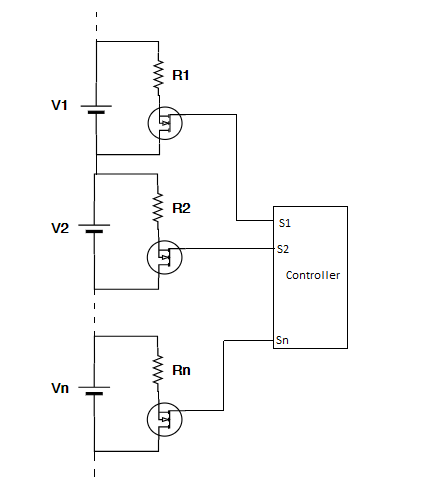
\includegraphics[]{Chapter2/Figures/switchedR.PNG}
    \caption{Switching  shunt resistor method}
\end{figure}
\section{Advantages of Passive Cell Balancing}

Passive cell balancing using switching shunt resistor method is chosen because of circuit design simplicity. Since it uses components like resistor and \acrshort{mosfet}'s has switches cost is less when compared with its active balance counterparts. And the system size will be less because of simple circuitry. The controller enables complete control over balancing so it gives designer the complete freedom to think of many algorithms possible and select a efficient one. Due its cost effectiveness, passive cell balancing is opted for the design.

\vspace{1cm}

This chapter gave an overview of different passive balancing techniques, its merits and demerits and possible applications. In the next chapter, design of the cell balancing circuit that was developed is discussed.  